% From mitthesis package
% Version: 1.01, 2023/07/04
% Documentation: https://ctan.org/pkg/mitthesis

\chapter{Experiments}
\section{Dropout Experiment}


\begin{figure}[ht]
   \centering
   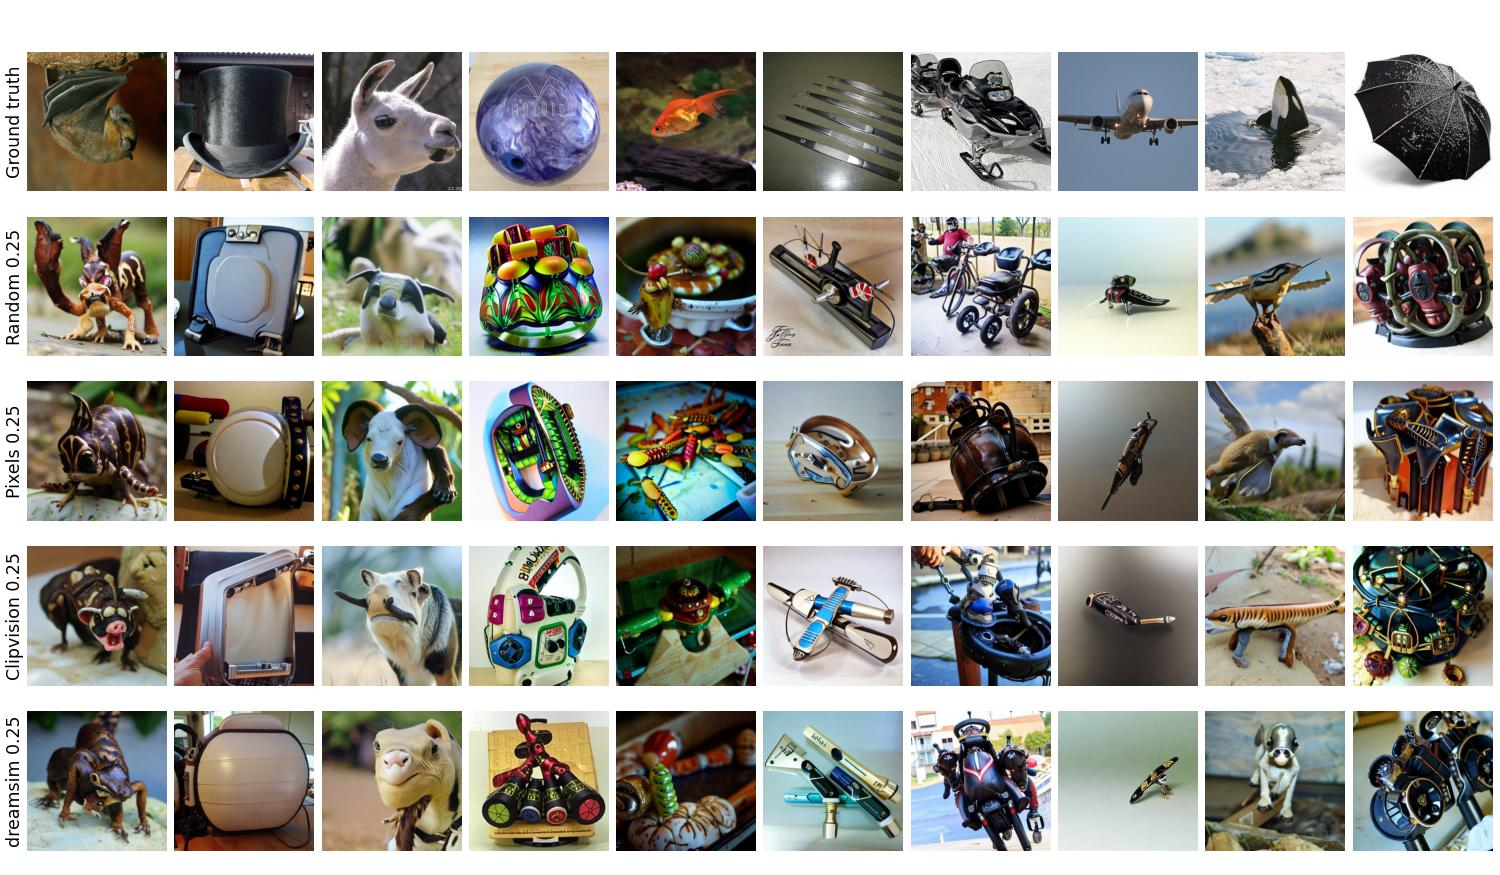
\includegraphics[width=1\textwidth]{plots/dropout_qual_eval_bd_test.JPEG}
   \caption{A nice image}\label{fig:dropout_qual_eval_bd_test}
\end{figure}

\begin{figure}[ht]
   \centering
   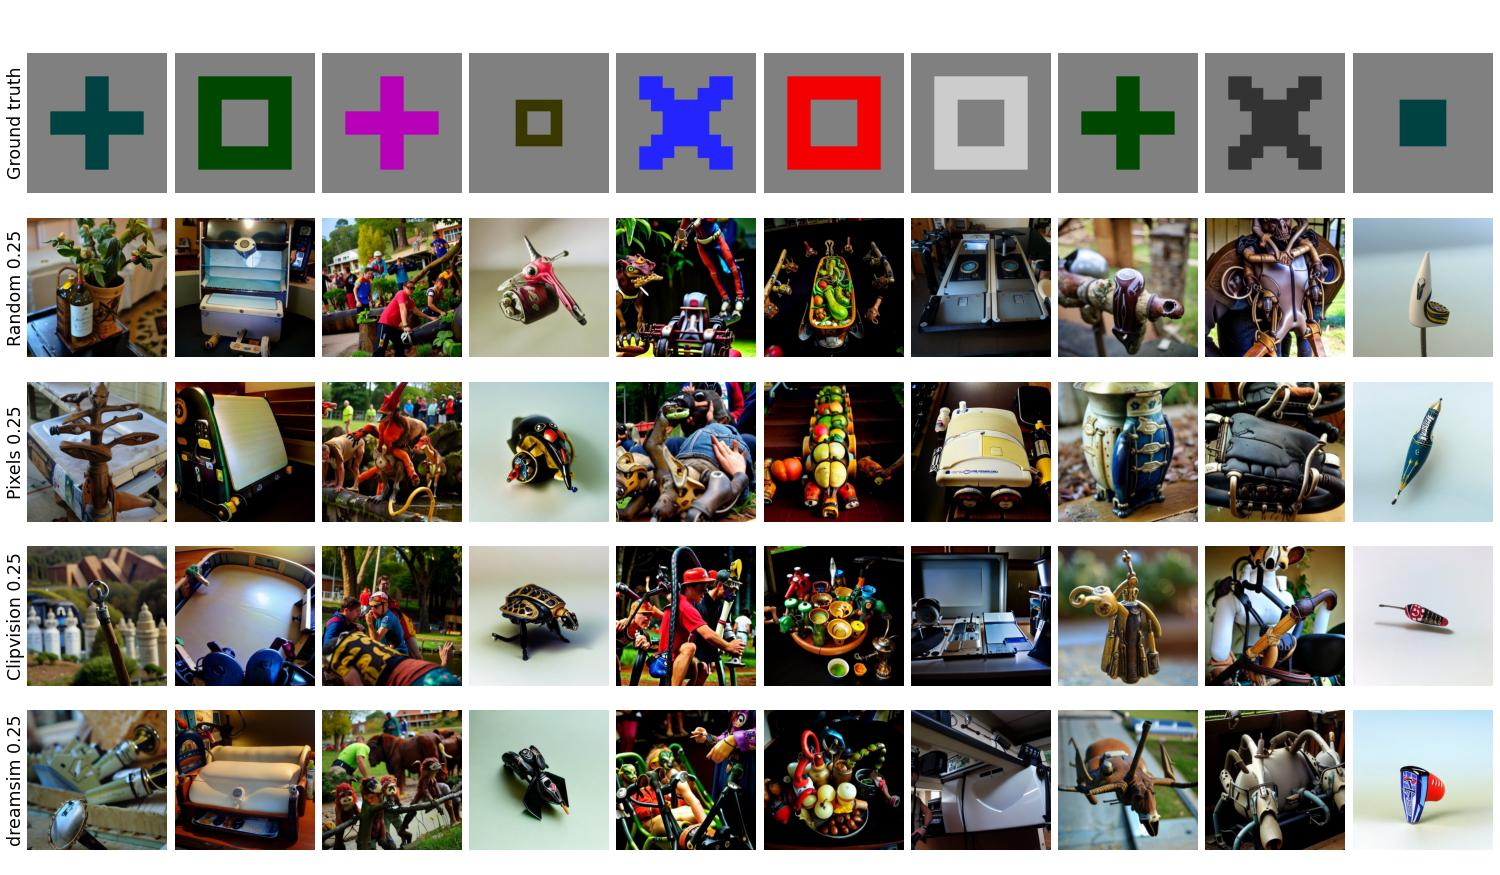
\includegraphics[width=1\textwidth]{plots/dropout_qual_eval_bd_art.JPEG}
   \caption{A nice image}\label{fig:dropout_qual_eval_bd_art}
\end{figure}

\section{Ai Captions}
\begin{figure}[ht]
   \centering
   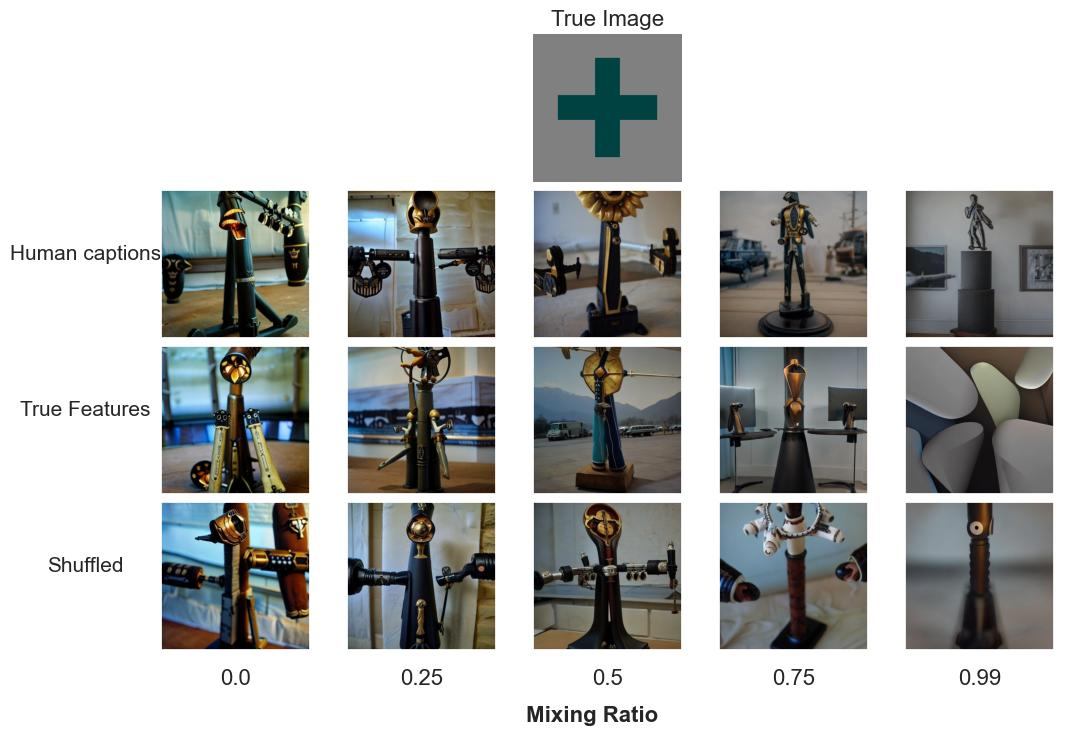
\includegraphics[width=1\textwidth]{plots/aicap_reconstruction_evolution_art_0.JPEG}
   \caption{AI-cap Reconstructions Artificial Shapes}\label{fig:aicap_reconstruction_evolution_art_0}
\end{figure}

\begin{figure}[ht]
   \centering
   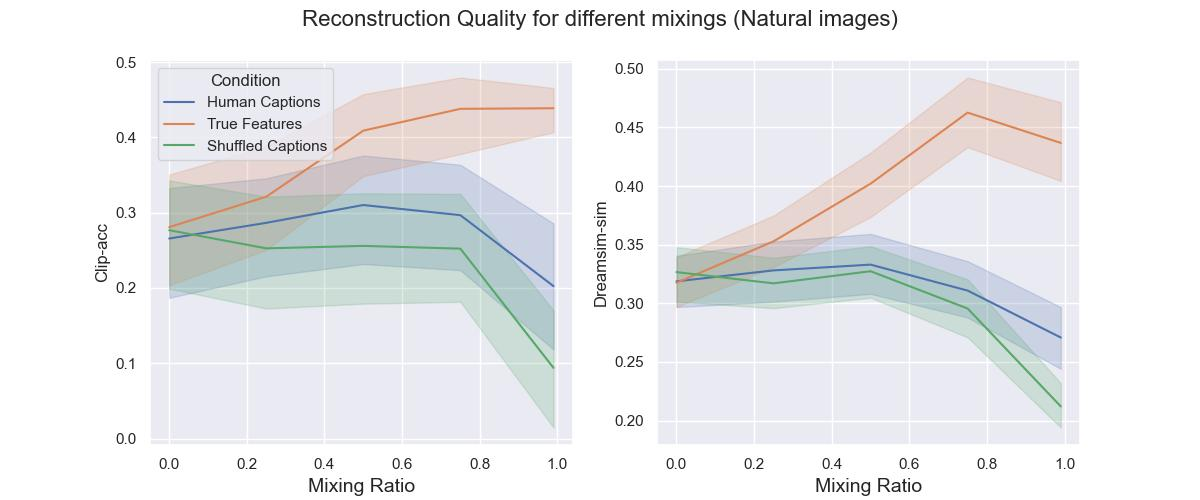
\includegraphics[width=1\textwidth]{plots/aicap_reconstruction_quant_evolution_test.JPEG}
   \caption{AI-cap Reconstructions Artificial Shapes}\label{fig:aicap_reconstruction_quant_evolution_test}
\end{figure}

\begin{figure}[ht]
   \centering
   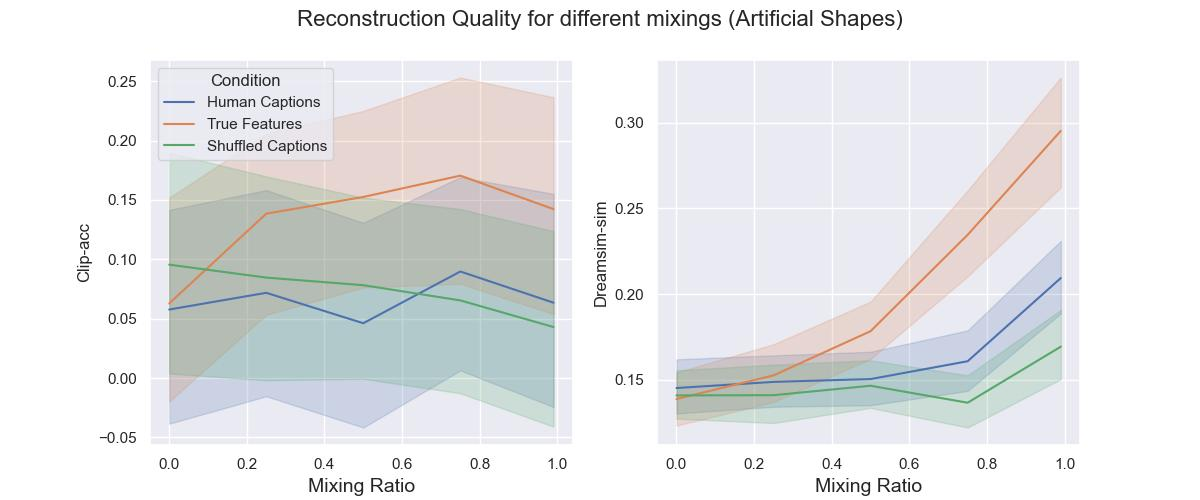
\includegraphics[width=1\textwidth]{plots/aicap_reconstruction_quant_evolution_art.JPEG}
   \caption{AI-cap Reconstructions Artificial Shapes}\label{fig:aicap_reconstruction_quant_evolution_art}
\end{figure}

\section{Perturbations}
\begin{figure}[ht]
    \centering
    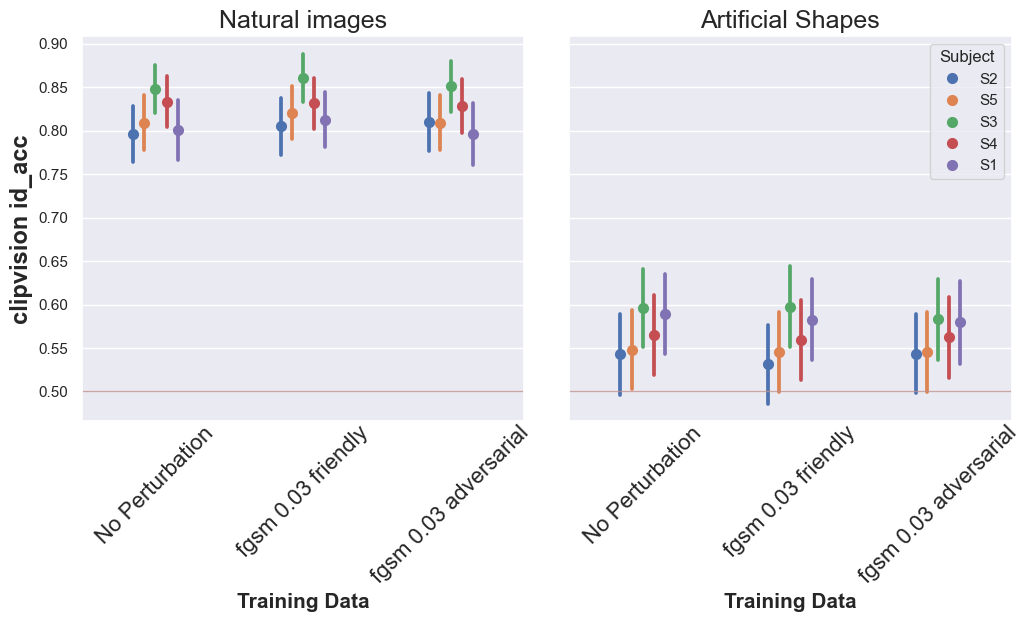
\includegraphics[width=1\textwidth]{plots/advpert_translator_fgsm_0.03.png}
    \caption{A nice image}\label{fig:advpert_translator_fgsm_0}
\end{figure}


\begin{figure}[ht]
    \centering
    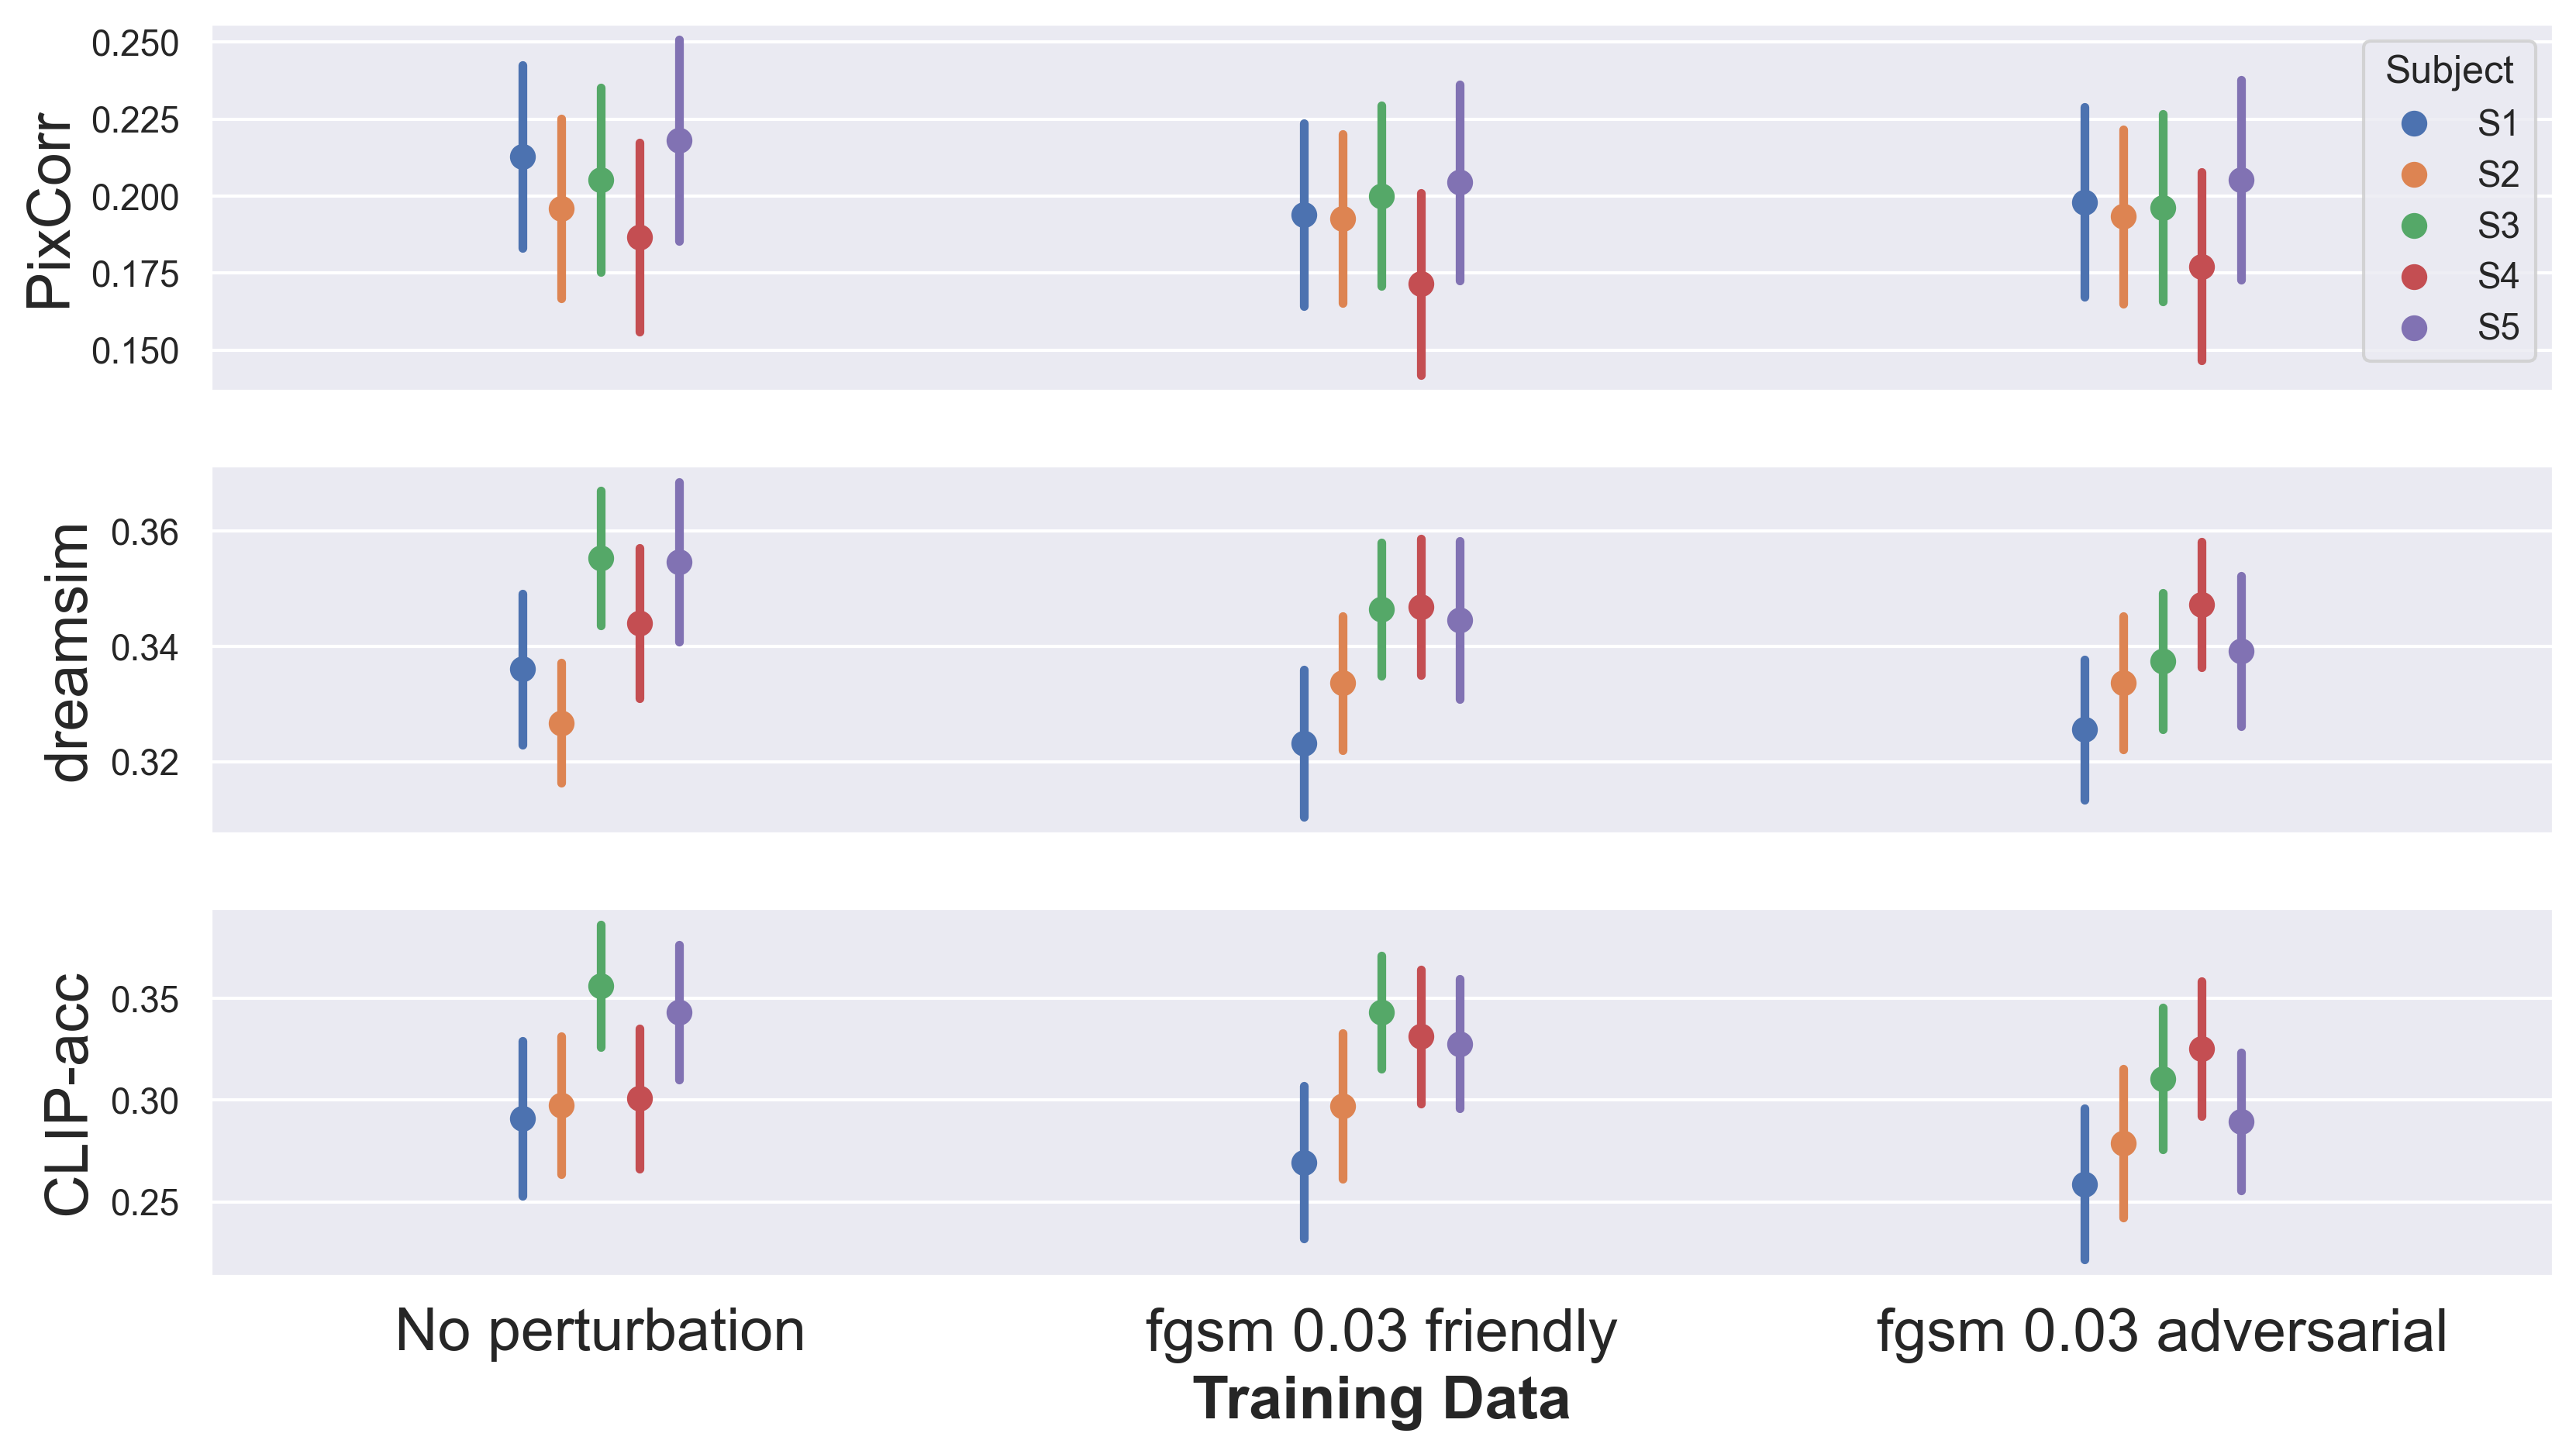
\includegraphics[width=1\textwidth]{plots/advpert_reconstruction_test_fgsm_0.03.png}
    \caption{A nice image}\label{fig:advpert_reconstruction_test_fgsm_0.03}
\end{figure}

\begin{figure}[ht]
    \centering
    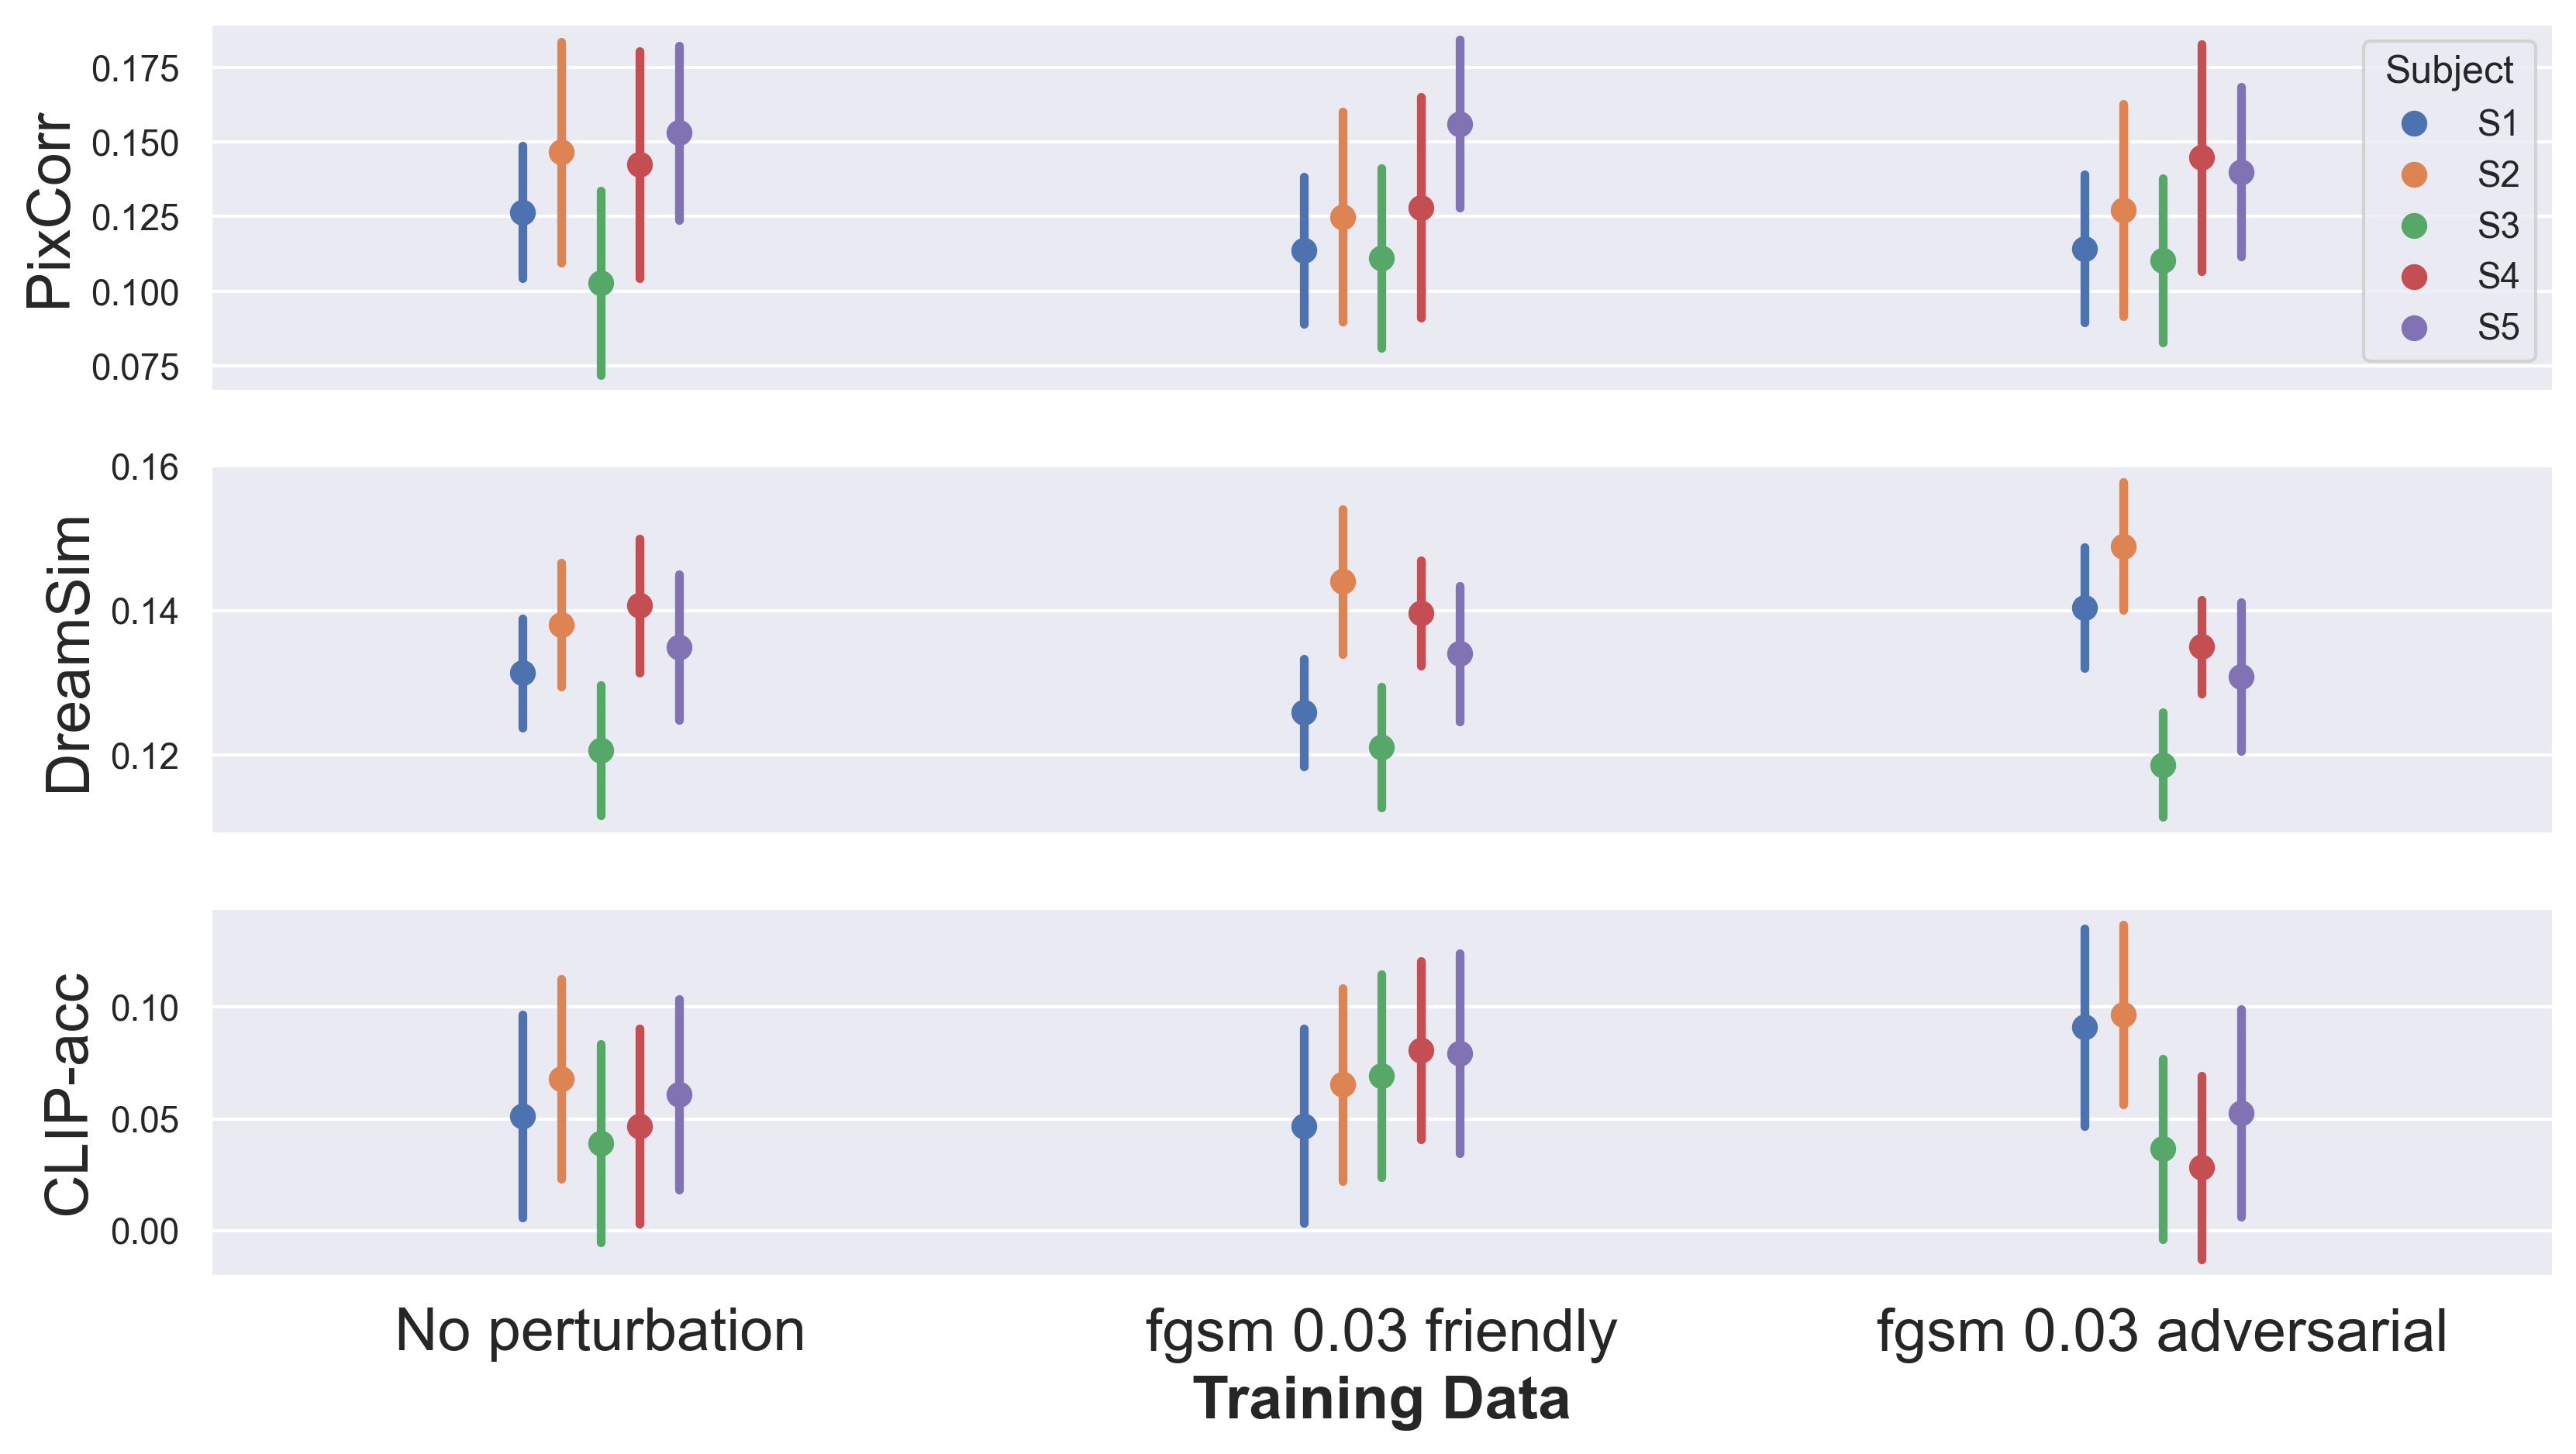
\includegraphics[width=1\textwidth]{plots/advpert_reconstruction_art_fgsm_0.03.png}
    \caption{A nice image}\label{fig:advpert_reconstruction_art_fgsm_0.03}
\end{figure}


% \chapter{Code listing}

% This example uses the \texttt{listings} package.

% \bigskip

% \lstdefinestyle{mystyle}{
%     backgroundcolor=\color{CadetBlue!15!white},   
%     commentstyle=\color{Red3},
%     numberstyle=\tiny\color{gray},
%     stringstyle=\color{Blue3},
%     basicstyle=\small\ttfamily,
%     breakatwhitespace=false,         
%     breaklines=true,                 
%     numbers=left,                    
%     numbersep=5pt,                  
%     showspaces=false,                
%     showstringspaces=false,
%     showtabs=false,                  
%     tabsize=2
% }%
% \lstset{language=[5.3]Lua,style={mystyle}}%

% \begin{lstlisting}
% function print_rate(kappa,xMin,xMax,npoints,option)
%      local c = 1-kappa*kappa
%      local croot = (1-kappa*kappa)^(1/2)
%      local logx = math.log(xMin)
%      local psi = 0
     
%      local xstep = (math.log(xMax)-math.log(xMin))/(npoints-1)
     
%      arg0 = math.sqrt(xMin/c)
%      psi0 = (1/c)*math.exp((kappa*arg0)^2)*(erfc(kappa*arg0)-erfc(arg0))
     
%      if option~=[[]] then
%   		 tex.sprint("\\addplot+["..option.."] coordinates{") 
%   		 -- addplot+ for color cycle to work
%      else
%   		 tex.sprint("\\addplot+ coordinates{")
%      end
%      tex.sprint("("..xMin..","..psi0..")")
     
%      for i=1, (npoints-1) do
%   		 x = math.exp(logx + xstep)
%   		 arg = math.sqrt(x/c)
%   		 karg = kappa*arg
%   		 if karg<5 then 
% 		 -- this break compensates for exp(karg^2), which multiplies the error in the erf approximation...
%   		    logpsi = -math.log(croot) + karg^2 + math.log(erfc(karg)-erfc(arg))
%   		    psi = math.exp(logpsi)
%   		 else
%   		    psi = (1/(karg) - 1/(2*(karg^3)) + 3/(4*(arg^5)) )/(1.77245385*croot)
%   		    -- this is the large x asymptote of the reaction rate
%   		 end
%   		 logx = math.log(x)
%   		 tex.sprint("("..x..","..psi..")")
%      end
%      tex.sprint("}")
% end
% \end{luacode*}
% \end{lstlisting}
